\section{Introduction}
\label{sec:intro}
\don{test don}
Combinatorial search problems are fundamental to computer science and artificial intelligence. Among the applications, we find logistics, scheduling, bioinformatics, and puzzle solving. 

The Futoshiki puzzle, a Japanese constraint satisfaction problem, serves as an excellent benchmark for evaluating algorithmic approaches to these challenges. Futoshiki requires filling an N×N grid with numbers from 1 to N while satisfying two constraint sets: the Latin Square property (each number appears exactly once per row and column) and inequality constraints between adjacent cells.

In the example given in \Cref{fig:futoshiki_example}, on the left-hand side it is easy to see that the only number defined is the '3' in the third column, the third row starting from the top right using 0 as the first index. We can also see the \textit{constraints} that are proposed from the problem (effectively differentiating Futoshiki from Sudoku as an extension of the \textit{Latin Square} puzzle). We have a total ordering fixed by the $`<`$ symbol, creating a chain of inequalities for which, defining F as the matrix and utilizing row-major indexing, e. g.
\[
\label{futoshiki_inequalities}
    F[3][1] < F[2][1] < F[2][2] < F[2][3] 
\]

Given this constraint, knowing that by the \textbf{Latin Square} property the values in the cell are NxN, where N is the number of cells on any side of the square, we therefore can be sure that $F[3][1] = 1$ and following the chain we end up with $F[2][3] = 4$.

\begin{figure}[H]
\centering
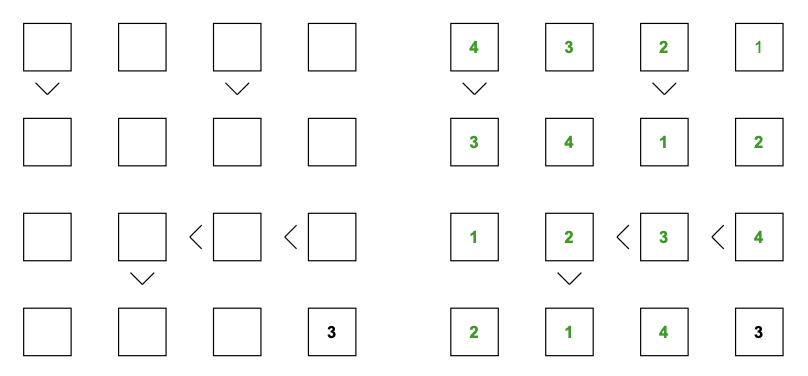
\includegraphics[scale=0.6]{imgs/futoshiki_example.png}
\caption{Example of a Futoshiki puzzle and its solved counterpart \cite{Sen2024Futoshiki}}
    \label{fig:futoshiki_example}
\end{figure}


From a high-level point of view, one could say it is similar to the more known \textit{Sudoku}, and it is true as both of these puzzles have as their main constraint the aforementioned \textit{Latin Square} property. The similarities among those are not only to be found at a conceptual level, but also when looking at it from a computer science point of view, specifically from a computational complexity standpoint, both of them lie in the family of NP-Complete problems. 

As for the complexity of Futoshiki, it is presented by Şen and Diner in \cite{Sen2024Futoshiki}. This means that while simple backtracking algorithms guarantee a solution, their exponential time complexity renders them impractical for large grids. In the aforementioned paper, a more sophisticated approach is presented: conceptually, Futoshiki puzzle can be transformed into a list coloring problem. This finding introduces a pre-coloring phase that propagates constraints to reduce possible values for each cell, significantly pruning the search space of the backtracking algorithm before the recursive search begins.


However, even with these optimizations, solving large or difficult puzzles is going to demand substantial computational resources. High-Performance Computing (HPC) makes it possible to overcome these limitations through parallelization across multiple processors. In this paper we present a comprehensive parallel solution for the Futoshiki puzzle that explores three distinct parallelization paradigms:

\begin{enumerate}
    \item \textbf{Distributed-Memory Parallelism (MPI):} \cite{MPIForum2021} Leveraging a dynamic master-worker approach to be able to scale across multiple nodes.
    \item \textbf{Shared-Memory Parallelism (OpenMP):} \cite{OpenMP2020} Exploiting multi-core architectures through task-based parallelism within a single node.
    \item \textbf{Hybrid Parallelism (MPI+OpenMP):} Combining both paradigms to maximize resource utilization.
\end{enumerate}

\sd{check after results}
the most important ones are:
\begin{itemize}
    \item An efficient sequential solver implementing the pre-coloring optimization algorithm presented in the Futoshiki paper as a performance baseline.
    \item An algorithm which dynamically performs fundamental puzzle solving before assigning to the different working units, based on the available parallelism, unlike work of the art solutions which employ a static work distribution.
    \item Three parallel implementations (MPI, OpenMP, Hybrid) with configurable task generation factors for workload tuning. For the last one, there is also the possibility of tweaking how much the solution should rely on MPI or omp.
    \item Comprehensive performance analysis including speedup, efficiency, and scalability metrics across all the solutions proposed.
\end{itemize}


\subsection{Outline of the paper}
We now present the overall structure of the paper: in \Cref{sec:related_work} we first present all of the necessary background information needed for the reader to understand the problem that we are tackling and the solution that we are proposing. We then proceed in \Cref{sec:solution} to showcase the solutions defined: we start from the sequential solution which is going to serve as a baseline, then we are going to move to the MPI and OpenMP version, and finally we are going to present the Hybrid solution and its configuration modes. In \Cref{sec:evaluation} we showcase under which hardware we are performing the evaluation and also we showcase how the different solutions presented can solve different puzzles. We then proceed to the conclusion of the work in \Cref{sec:conclusion} and finally we present the needed \Cref{sec:future_work}.